\section{Fonctionnement de HTTP/HTTPS}

%%%%%%%%%%%%%%%%%%%%%%%%%%%
%  Fonctionnement de HTTP %
%%%%%%%%%%%%%%%%%%%%%%%%%%%

\begin{frame}{Fonctionnement de HTTP}
    Procotole de communication client-serveur \\
    Le client demande une ressource à un serveur via une requête HTTP \\
    % Généralement une page html
    Le serveur envoie au client la ressource demandée en réponse \\
    Un navigateur web permet d'automatiser ce processus \\
    De plus ce dernier permet d'afficher la page avec la mise en forme html/css

\end{frame}

%%%%%%%%%%%%%%%%%%%%%%%%%%%
%  Exemple de HTTP        %
%%%%%%%%%%%%%%%%%%%%%%%%%%%

\begin{frame}{Exemple d'une requête HTTP}
    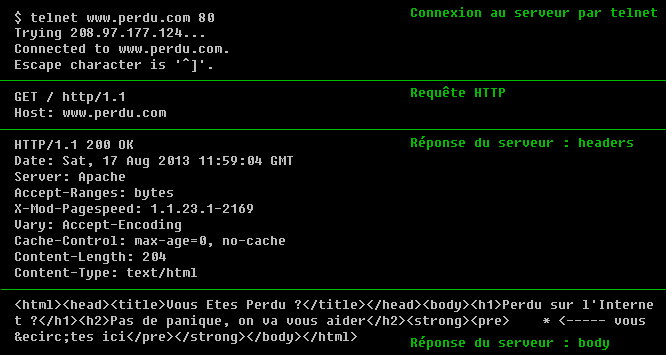
\includegraphics[width=\linewidth]{../medias/perdu.png}
    % Faire une petite démo en live (avec la même requête)
\end{frame}

%%%%%%%%%%%%%%%%%%%%%%%%%%%
%  HTTPS                  %
%%%%%%%%%%%%%%%%%%%%%%%%%%%

\begin{frame}{HTTPS : la version chiffrée de HTTP}
    S pour secure \\
    C'est un deuxième protocole qui est rajouté par dessus HTTP \\
    Historiquement SSL, aujourd'hui remplacé par TLS \\
    Applique un chiffrement sur toute la communication HTTP \\

    Limitation : un attaquant peut toujours voir l'IP/port de destination (nécessaire pour TCP/IP)
\end{frame}


%%%%%%%%%%%%%%%%%%%%%%%%%%%
%  Certificats            %
%%%%%%%%%%%%%%%%%%%%%%%%%%%

\begin{frame}{Gestion des certificats}
  -> Permet d'authentifier la communication \\
  -> Sur internet, cela sert essentiellement à s'assurer de l'identité du serveur \\
  -> Nécessité d'une authorité de certification (un tiers) \\
\end{frame}

%%%%%%%%%%%%%%%%%%%%%%%%%%%
%  TLS                    %
%%%%%%%%%%%%%%%%%%%%%%%%%%%

\begin{frame}{Le protocole SSL/TLS}
  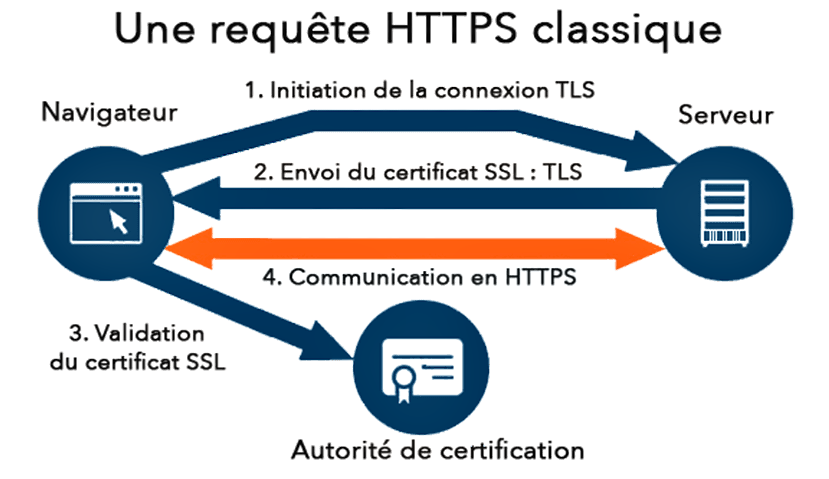
\includegraphics[width=\linewidth]{../medias/protocole-tls.png}
\end{frame}
